\begin{figure}[h]
    \centering
    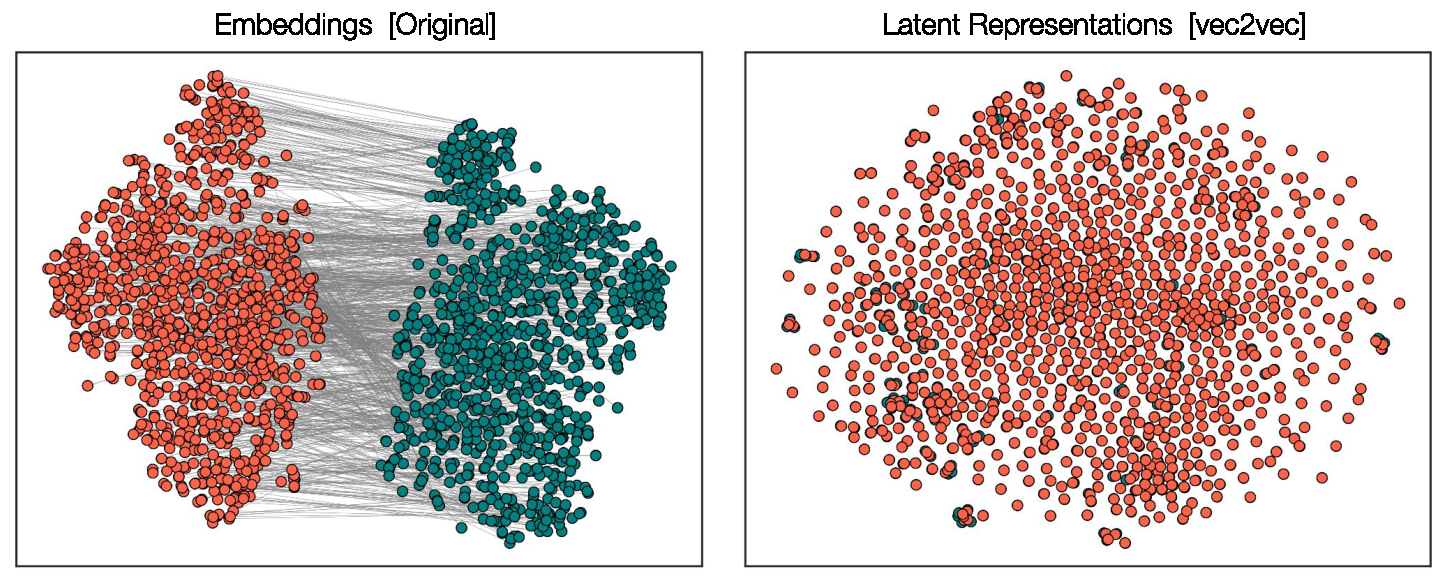
\includegraphics[width=0.8\linewidth]{ims/universal2.pdf}
    \caption{Left: input embeddings from different model families (T5-based GTR \citep{ni2021gtr} and BERT-based GTE \citep{li2023gte}) are fundamentally incomparable. Right:
    given unpaired embedding samples from different models on different texts, our model learns a latent representation where they are closely aligned.}
    \label{fig:main}
\end{figure}


\begin{figure}[t]
    \centering
    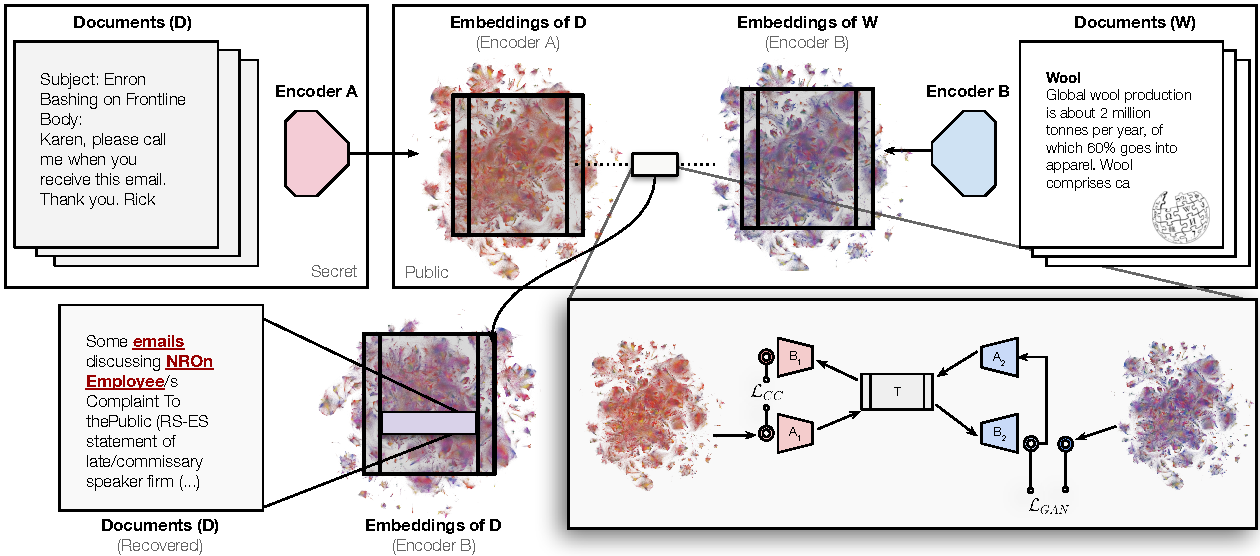
\includegraphics[width=0.85\linewidth]{ims/diagram.pdf}
    \caption{Given only a vector database from an unknown model, \atk{} translates the database into the space of a known model using latent structure alone. Converted embeddings reveal sensitive information about the original documents, such as the topic of an email (pictured, real example).}
    % https://docs.google.com/drawings/d/15lO_xIOkSc-jI75ThhHp4K_mFUQFW0nI--rZyht2avg/edit?usp=sharing
    \label{fig:architecture}
\end{figure}
\section{Introduction}

Text embeddings are the backbone of modern NLP, powering tasks like retrieval, RAG, classification, and clustering.  There are many embedding models trained on different datasets, data shufflings, and initializations.  An embedding of a text encodes its semantics: a good model maps texts with similar semantics to vectors close to each other in the embedding space.    Since semantics is a property of text, different embeddings of the same text should encode the same semantics.  In practice, however, different models encode texts into completely different and incompatible vector spaces.

% Semantics is a property of input text, and should be invariant to the embedding model chosen. However, many neural embedding models exist. These models are trained on different datasets, data shufflings, and initializations. This inconsistency has produced a world of embedding models trained on similar or identical datasets encoding the same semantics in completely different and incompatible spaces \Cref{fig:main}.

% Prior work  \citep{huh2024platonicrepresentationhypothesis} has proposed that models trained on the same modality share inevitable similarities due to their shared underlying reality (i.e. the world we live in). Another line of research develops systems to quantify this similarity between representation spaces \citep{maiorca2024latentspacetranslationsemantic, moschella2023relativerepresentationsenablezeroshot, moayeri2023texttoconceptandbackcrossmodel, norelli2023asifcoupleddataturns}. These works have achieved remarkable results including zero-shot stitching, substitution, and multi-modal adaptation without training. However, all of these methods rely on at least a small amount of paired data between the two modalities of interest; efforts to reduce the number of pairs required have proven difficult \citep{cannistraci2023bootstrappingparallelanchorsrelative}.

% \rj{The jump between these two paragraphs feels a little abrupt. Also we should converge on a wording of the hypothesis. I think we should avoid the word 'mapping'}

The Platonic Representation Hypothesis \citep{huh2024platonicrepresentationhypothesis} conjectures that all image models of sufficient size have the same latent representation.  We propose a stronger, constructive version of this hypothesis for text models: the universal latent structure of text representations can be learned and, furthermore, harnessed to translate representations from one space to another without any paired data or encoders.

In this work, we show that the Strong Platonic Representation Hypothesis holds in practice.  Given unpaired examples of embeddings from two models with different architectures and training data, our method learns a latent representation in which the embeddings are almost identical (\Cref{fig:main}).

We draw inspiration from research on aligning word embeddings across languages \citep{xing2015normalized, conneau2018wordtranslationparalleldata, grave2018unsupervisedalignmentembeddingswasserstein, chen2018unsupervisedmultilingualwordembeddings} and unsupervised image translation
\citep{liu2018unsupervisedimagetoimagetranslationnetworks,zhu2020unpairedimagetoimagetranslationusing}. Our \atk{} method uses adversarial losses and cycle consistency to learn to encode embeddings into a shared latent space and decode with minimal loss.  This makes unsupervised translation possible.  We use a basic adversarial approach with vector space preservation \citep{mrksic2016counterfittingwordvectorslinguistic} to learn a mapping from an unknown embedding distribution to a known one.

% Trained on as few as 50K unpaired samples from each model, 
\atk{} is the
\textbf{first method to successfully translate embeddings from the space of one model to another without any paired data.}
\atk{}
translations achieve cosine similarity as high as $0.92$ to the ground-truth vectors in their target embedding spaces and perfect matching on over $8000$ shuffled embeddings (without access to the set of possible matches in advance). 

To show that our translations preserve not only the relative geometry of embeddings but also the semantics of underlying inputs, we extract information from them using zero-shot attribute inference and inversion, without any knowledge of the model that produced the original embeddings!

% In one case, we are able to take a database of 100K vectors from an unknown embedding model and learn an unsupervised mapping to a known embedding space. Given our translated embeddings are then able to perform attribute extraction as well as inversion without any paired data, without making any function calls to the unknown encoder, and crucially \textit{without knowing anything about the model used to produce the embeddings}. \rj{1M (although I think the ablations will show this is true for 100K and maybe 50K).} \rj{Also confused by what the first sentence is adding--statement on data amount? Why is it "in once case"--don't we do that for all? Second sentence seems incomplete?}

% To demonstrate that our translation not only preserves relative geometry of embedding vectors (measured via cosine similarity) but also semantics, we carry out several experiments to demonstrate that we can use translation to extract essential semantic information about the text encoded in the source embeddings. We are able to perform classification on tweet embeddings and extract sensitive information from emails.

